\documentclass[a4paper,12pt]{article}

% Font
\usepackage[T1]{fontenc}
\usepackage{gentium}

% Math packages
\usepackage{amsmath}
\usepackage{amsfonts}
\usepackage{amssymb}
\usepackage{amsthm}
\usepackage{bm}

% Define symbol shortcuts
\newcommand{\cc}{\mathcal{C}}
\newcommand{\dd}{\mathcal{D}}
\newcommand{\hh}{\mathcal{H}}
\newcommand{\xx}{{\bm x}}
\newcommand{\yy}{{\bm y}}

% Math environment
\newtheorem*{thm}{Theorem}

% Better list management:
% - vertical spacing in lists
% - items in lists start with dash not bullet point.
\usepackage{enumitem}
\setlist{label=\textemdash,
  itemsep=0pt, topsep=3pt, partopsep=0pt} 

% Include graphics
\usepackage{graphicx}
\usepackage{subcaption}

% Page format 
\usepackage[top=2cm,left=2cm,right=2cm,bottom=2cm]{geometry}
\usepackage{float}

\begin{document}
%%% HEADER
\raisebox{0.6in}[0in]{\makebox[\textwidth][r]{\it Unproofed version }}
\vspace{-0.7in}

\begin{center}
\bf\large MA2823 : Foundations of Machine Learning \\
Chapter 5 : Linear Regression
\end{center}

\noindent
Lecturer : Chlo\'e-Agathe Azencott   
\hfill
Scribes : Emilie Leblanc, Antoine Salon, Hippolyte Jacomet 

\noindent
\rule{\textwidth}{1pt}

\medskip

%%% NOTES START HERE
In this chapter we will see how to :
\begin{itemize}
\item define parametric methods ;
\item define the maximum likelihood estimator and compute it
for Bernoulli, multinomial and Gaussian densities ;
\item define the Bayes estimator and compute it for normal
priors ;
\item compute the maximum likelihood estimator / least-square
fit solution for linear regression ;
\item compute the maximum likelihood estimator for logistic
regression.
\end{itemize}

\section{Parametric methods}

In this chapter we would like to define different ways of building estimators that are part of a statistical model, and how to assess their performances.

\paragraph{Definitions and notations} Let us consider a training set of $n$ $p$-dimensional vectors denoted by $\mathcal{X}=\{x^i\}_{i=1,\dots,n}$, and let's assume that each of these observation follows a law of probability given a parameter $\theta$. 

\[
\forall i \in [1,\dots,n],\ \xx^{i}\sim{}p(\xx|\theta)
\]\\
The {\em parametric estimation} consists in {\em assuming} a form for $p(\xx|\theta)$ and then {\em estimating} the parameter $\theta$ using our training set $\mathcal{X}$. \\
For example, if we assume that the observations of our training set follow a Gaussian distribution $p(x_{j}|\theta_j)\sim{}\mathcal{N}(\mu_j,{\sigma_j}^2)$ our goal would be to estimate the parameter $\theta=\{\mu_1,\sigma_1,\dots,\mu_p,\sigma_p\}$. \\
\\
To achieve that goal, the observations of the training set $\xx^i$ are usually assumed to be {\em independent and identically distributed} (i.i.d.). \\

In the following sections we sill study two different methods to estimate the parameters : the {\em maximum likelihood estimation} and the {\em Bayes estimation}.


\subsection{Maximum likelihood estimation}

This first method relies on the idea that $\theta$ should maximize the likelihood for $\mathcal{X}$ to be drawn from the law of probability we chose in our model.

\paragraph{Likelihood and log-likelihood} We call {\em likelihood of} $\theta$ given $\mathcal{X}$ the function : $\ell(\cdot{}|\mathcal{X}) : \theta \mapsto p(\mathcal{X}|\theta).$\\
In the case of an i.i.d. sample $\mathcal{X}$, this becomes :

\[\ell(\theta|\mathcal{X})=p(\mathcal{X}|\theta)=p(\xx^1|\theta)p(\xx^2|\theta)\dots{}p(\xx^p|\theta)\] \\
It is often useful to also consider the {\em log-likelihood}, simply defined by $\mathcal{L} (\cdot{}|\mathcal{X}) : \theta \mapsto \log \ell(\theta|\mathcal{X})$, which in our previously mentioned case becomes :
\[\mathcal{L}(\theta|\mathcal{X})=\log{p(\xx^1|\theta)}+\dots{}+\log{p(\xx^n|\theta)}\]
\\
Given these two functions, we will then try to find the estimator that maximizes them, called the {\em maximum likelihood estimator} or MLE, and defined by :

\[\hat{\theta}=\arg\underset{\theta}\max \  \ell(\theta|\mathcal{X})=\arg\underset{\theta}\max \  \mathcal{L}(\theta|\mathcal{X})\]\\


Let us now look at these MLE for Bernoulli, Multinomial and Normal laws.

\subsubsection{Bernoulli density}

Such a law corresponds to observations that reflect two states of either failure or success (think of a coin toss for example), and thus let us consider a data set $\mathcal{X}=\{x^i\}_{i=1,\dots,n}$ with  $x^i\in\{0,1\}$ $\forall i\in[1,\dots,n]$.\\
\\
The Bernoulli density is given by $P(X=x|p_0)={p_0}^{x}(1-p_0)^{(1-x)}$, let us try to find the MLE $\ \hat{p_0}$ of the parameter $p_0$.\\
\\
We first compute the log-likelihood :

\[\mathcal{L}(p_0|\mathcal{X})=\log{P(\mathcal{X}|p_0)}=\sum_{i=1}^n\left(x^i\log p_0 + (1-x^i)\log{(1-p_0)}\right)\]
This is a concave function which we can easily maximize by setting its gradient to 0 :

\[\frac{\sum_{i=1}^nx^i}{\hat{p_0}}-\frac{n}{(1-\hat{p_0})}+\frac{\sum_{i=1}^nx^i}{(1-\hat{p_0})}= 0
\]
Which yields the MLE of $p_0$ :

\[\hat{p_0}=\frac{1}{n}\sum_{i=1}^nx^i\]


\subsubsection{Multinomial density}

Let us consider $K$ mutually exclusive and exhaustive classes. The probability for each class to occur is $p_k$, with $\sum_{k=1}^Kp_k=1$. We represent these classes with $K$ indicator variables $x_1, x_2, \dots, x_K$ knowing 
\[
    x_k= 
\begin{cases}
    1& \text{if the outcome is class } k\\
    0              & \text{otherwise}
\end{cases}
\]
The joint probability distribution is given by :
\[P(x_1,x_2,\dots,x_K)=\displaystyle\prod_{k=1}^{K}p_k^{x_k}\]\\
\\
Let us compute the MLE $\bm{\hat{p}}=(\hat{p_1},\dots,\hat{p_K})$. The observations are i.i.d. thus the log-likelihood looks dramatically like :
\\
\[\mathcal{L}(\bm p|\mathcal{X})=\sum_{i=1}^n\sum_{k=1}^K x_k^i\log p_k
\]\\
And we now have to maximize it under the constraint $\displaystyle\sum_{k=1}^Kp_k=1$.\\
We must call on to a Lagrange multiplier $\lambda$ and define the Lagrangian function 
\[\mathcal{F} : (\bm p, \lambda) \mapsto \mathcal{L}(\bm p|\mathcal{X})-\lambda \left(\sum_{k=1}^Kp_k - 1\right)\]
Setting its gradient to zero gently yields a system of equations from which we are happy to learn that $\lambda=n$ and consequently that

\[\hat{p}_k=\dfrac{1}{n}\displaystyle\sum_{i=1}^nx_k^i\ \ \ \ \ \ \ \ \forall k \in [1,\dots,K]\]


\subsubsection{Gaussian distribution}

Let us now assume that our observations $x^i$ are i.i.d. following a Gaussian distribution, i.e. : 

$\forall i \in [1,\dots,n]$,
\[x^i\sim\mathcal{N}(\mu,\sigma^2)\]

\[p(x^i|\mu,\theta)=\dfrac{1}{\sqrt[]{2\pi}\sigma}\exp\left[-\frac{(x^i-\mu)^2}{2\sigma^2}\right]\]
\\

Setting the gradient of the log-likelihood to zero yields the estimators :

\[ \hat{\mu} = \frac{1}{n} \sum_{i=1}^nx^i\]
\[ \hat{\sigma}^2 = \frac{1}{n} \sum_{i=1}^n (x^i-\hat{\mu})^2\]

\subsection{Bias-variance trade-off}

We can assess the performance of the estimator (be it obtain through MLE or another method) by computing the {\em mean squared error} or MLE, defined by :

\[\mbox{MSE}(\hat{\theta}) = \mathbb{E}[(\hat{\theta}-\theta_0)^2]\]

\paragraph{Bias-variance trade-off} Let us try to link this MSE to two previously known notions that help characterize our estimator, the variance and the bias. As a reminder, the {\em bias} of an estimator is the difference between this estimator's expected value and the true value of the parameter being estimated : $\mbox{Bias}(\hat{\theta})=\mathbb{E}[\hat{\theta}]-\theta_0$. 

\begin{align*}
\mbox{MSE}(\hat{\theta}) &= \mathbb{E}[(\hat{\theta}-\theta_0)^2]\\  
&= \mathbb{E}\left[(\hat{\theta}-\mathbb{E}[\hat{\theta}])^2+2\hat{\theta}\mathbb{E}[\hat{\theta}]-\mathbb{E}[\hat{\theta}]^2-2\hat{\theta}\theta_0+\theta_0^2\right]\\
&=\mbox{Var}(\hat{\theta})+\mathbb{E}[\hat{\theta}]^2-2\mathbb{E}[\hat{\theta}]\theta_0+\theta_0^2\\
&=\mbox{Var}(\hat{\theta})+\mbox{Bias}^2(\hat{\theta})
\end{align*}\\
We see that the MSE is a balance between these two positive expressions, hence the idea of a {\em bias-variance trade-off}. We understand that a biased estimator may achieve better MSE than an
unbiased one, as illustrated below :

\begin{center}
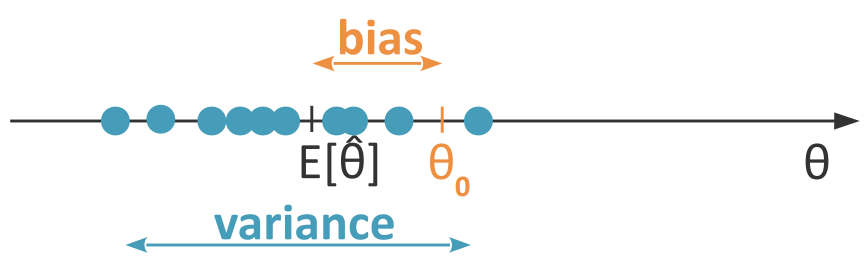
\includegraphics[width=100mm]{biasvariance.png}
\end{center}

\subsection{Bayes estimator}
From now on let us study another way of building an estimator, using Bayes rule which in its general form is :
\[P(C|\xx)  = \dfrac{P(C)p(\xx|C)}{p(\xx)}\]\\
Here we choose to treat $\theta$ as a random variable with a given prior distribution $p(\theta)$. Considering an observation-set $\mathcal{X}$, the Bayes rule yields :

\[p(\theta|\mathcal{X})=\frac{p(x|\theta)p(\theta)}{p(\mathcal{X})}\]\\
\\
We define the {\em Bayes estimate} as the conditional expected value of $\theta$ given our data set $\mathcal{X}$ :
\[\hat{\theta}_{\mbox{Bayes}}=\mathbb{E}[\theta|\mathcal{X}]=\int{\!\theta p(\theta|\mathcal{X})d\theta}\]\\
\\
Here's a reminder of the estimates we have previously seen :\\

{\em Maximum a posteriori} estimate :
\[\hat{\theta}_{\mbox{MAP}}=\arg\underset{\theta}\max \  p(\theta|\mathcal{X})\]

{\em Maximum likelihood} estimate :
\[\hat{\theta}_{\mbox{MLE}}=\arg\underset{\theta}\max \  p(\mathcal{X}|\theta)\]\\


\subsubsection{Bayes estimator for normal priors}

Let us consider $n$ i.i.d. data points $x^i$ following a normal law, $x^i\sim\mathcal{N}(\theta,\sigma^2)$ and let's assume that $\theta$ is of Gaussian prior distribution : $\theta\sim\mathcal{N}(\mu,\sigma_0^2)$.\\
\\
We know that the MLE of $\theta$ is its sample mean : $\hat{\theta}_{\mbox{MLE}} = \frac{1}{n} \sum_{i=1}^nx^i$ and we would like to compare it to its Bayes estimator.\\
\\
After a long and troublesome computation, a quick look at $p(\theta|\mathcal{X})$ shows us that it follows a normal distribution with mean $m$ and variance $s^2$ :

\[m = \frac{n\hat{\theta}_{\mbox{MLE}}\sigma^2+\mu\sigma_0^2}{n\sigma^2+\sigma_0^2}
\]

\[s^2 = \frac{\sigma^2\sigma_0^2}{n\sigma^2+\sigma_0^2}
\]\\
\\
Knowing that :
\[\mathbb{E}[\theta|\mathcal{X}]=m\]
We can conclude with :
\[\hat{\theta}_{\mbox{Bayes}}=\frac{\frac{n}{\sigma_0^2}}{\frac{n}{\sigma_0^2}+\frac{1}{\sigma^2}}\hat{\theta}_{\mbox{MLE}}+\frac{\frac{1}{\sigma^2}}{\frac{n}{\sigma_0^2}+\frac{1}{\sigma^2}}\mu
\]\\
\\
It is interesting to notice that when n increases, $\hat{\theta}_{\mbox{Bayes}}$ gets closer to the sample average (uses
information from the sample) and When $\sigma$ is small, $\hat{\theta}_{\mbox{Bayes}}$ gets closer to $\mu$ (little uncertainty
about the prior). 

\section{Linear regression}

The goal of a {\em linear regression} is to approximate the law followed by our data \(\textit{y}\) by a linear combination of observed variables \(\xx\) such as :
\[ f(\xx|\beta)= \displaystyle\sum_{j=1}^{p} \beta_j*x_j + \beta_0\]
with \(\xx^i \in \mathbb{R}^p\)  and \(\textit{y}^i \in \mathbb{R}\) and noting \(\dd = {\{\xx^i,\textit{y}^i\}}_{\textit{i}=1,..,\textit{n}}\). 
\begin{center}
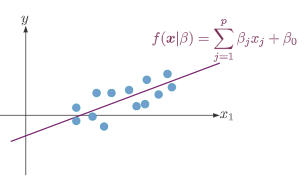
\includegraphics[width=100mm]{linear_regression_example.png}
\end{center}

We assume that the error \(\epsilon\) we have while doing a regression is \textbf{Gaussian distributed}. Therefore, with \(y = g(\xx) + \epsilon \),  \(f(\xx|\beta)\) being \(g\)'s estimator, we have : 
\begin{center}
\(\epsilon = y - g(\xx)\) and \(\epsilon\sim{}\mathcal{N}(0,{\sigma}^2)\)
\end{center}

We therefore have our \(\dd = {\{\xx^i,\textit{y}^i\}}_{\textit{i}=1,..,\textit{n}}\) observations (the blue dots), the linear regression obtained \(\mathbb{E}(y|x) = \beta*x + \beta_0\) and, for each new \(x^*\) point, we can compute the hypothetical \(y^* = \mathbb{E}(y|x^*)\) value and the corresponding error \(\epsilon^* \) and confidence interval given by \(p(y|x^*)\) since : 
\[p(y|\xx)\sim{}\mathcal{N}(f(\xx|\beta),{\sigma}^2)\]
\begin{center}
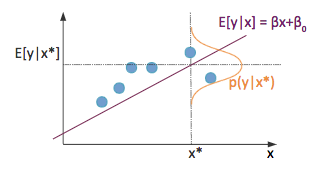
\includegraphics[width=100mm]{LR_2.png}
\end{center}

\subsection{Maximum likelihood estimation under Gaussian noise}

We are now going to use the \textit{maximum likelihood estimation} in order to find the best linear regression possible to fit the data and predict new points. \\
\\
Under Gaussian noise, considering i.i.d. observations and with \(p(y|\xx)\sim{}\mathcal{N}(f(\xx|\beta),{\sigma}^2)\), the log-likelihood defined earlier becomes : 
\begin{align*}
\mathcal{L}(\beta|\dd) &= \log\displaystyle\prod_{i=1}^{n} p(y^i|\xx^i) + \log\displaystyle\prod_{i=1}^{n} p(\xx^i) \\  &= \log \left(\displaystyle\prod_{i=1}^{n} \frac{1}{\sqrt{2\pi}\sigma}*exp\left[ - \frac{(y^i - f(\xx^i|\beta))^2}{2\sigma^2} \right] \right ) + Cte  \\
& = Cte - \frac{1}{2\sigma^2} \displaystyle\sum_{i=1}^{n} (y^i - f(\xx^i|\beta))^2
\end{align*}
Since \(\log\displaystyle\prod_{i=1}^{n} p(\xx^i)\) is independent of \(\beta\), its value is added to a term \(Cte\) along with others. \\
Assuming Gaussian error, maximizing the likelihood \(\mathcal{L}(\beta|\dd)\) is therefore equivalent to minimizing the sum of squared residuals \(\displaystyle\sum_{i=1}^{n} (y^i - f(\xx^i|\beta))^2\). 
This expression of the residual sum of squares can also be written in matrix form : 
\begin{align*}
RSS(\beta) &= \displaystyle\sum_{i=1}^{n} (y^i - f(\xx^i))^2 \\  &= \displaystyle\sum_{i=1}^{n} \left( y^i - \beta_0 - \displaystyle\sum_{j=1}^{p} x_j^i \beta_j \right)^2 \\
& = (y - \textbf{\textit{X}} \beta)^T * (y - \textbf{\textit{X}} \beta)
\end{align*}
with \(\textbf{\textit{X}} = \left( \begin{array}{ccccc}
1 & x_1^1 & x_2^1 & ... & x_p^1 \\
1 & x_1^2 & x_2^2 & ... & x_p^2 \\
. & . & . & ... & .\\
. & . & . & ... & .\\
. & . & . & ... & .\\
1 & x_1^n & x_2^n & ... & x_p^n \end{array} \right) \). 
Here, we added a vector \(\left( \begin{array}{c}
1 \\
1 \\
.\\
. \\
. \\
1 \end{array} \right)\) to \({\{\xx^i\}}_{\textit{i}=1,..,\textit{n}}\) in  \(\textbf{\textit{X}}\)'s expression in order to compute the scalar \(\beta_0\). \\
\\ 
Historically, the use of the residual sum of squares minimization can be attributed to Carl Friedrich Gauss (to predict the location of Ceres) and Adrien Marie Legendre. 
\\
\\
\textbf{In this method, under which conditions is \(\beta\)'s estimator unique ? }
\\

\begin{itemize}
\item 
In order to minimize \(RSS(\beta)\), \(\textbf{\textit{X}}\) must have a full column rank, hence \(\textbf{\textit{X}}^T\textbf{\textit{X}}\) \textit{invertible}. In this case, the \(\beta\) minimizing \(RSS(\beta)\) is : 
\[\hat{\beta} = (\textbf{\textit{X}}^T\textbf{\textit{X}})^{-1} \textbf{\textit{X}}^T y\]
\item 
If \(\textbf{\textit{X}}^T\textbf{\textit{X}}\) is not invertible (or \textit{rank-deficient}), we can use its pseudo-inverse. However, when doing so, we must keep in mind that the solution is \textit{not} unique. \\ A pseudo-inverse of\textbf{ A} is a matrix \textbf{G} such as \textbf{AGA = A}.
\end{itemize}
 


\subsection{Gauss-Markov Theorem}

\textbf{Gauss-Markov Theorem :} Under the assumption that \(\epsilon\sim{}\mathcal{N}(0,{\sigma}^2)\), the least-squares estimator of \(\beta\) is its best linear unbiased estimator. This Best Linear Unbiased Estimator is unique if \(\textbf{\textit{X}}^T\textbf{\textit{X}}\) is invertible. We call it the "\textit{BLUE}". 
\\
\\
Indeed, with \(\hat{\beta} = (\textbf{\textit{X}}^T\textbf{\textit{X}})^{-1} \textbf{\textit{X}}^T y\), we can show that (demonstration of the Gauss-Markov Theorem) : 
\begin{center}
\(\forall \beta^*\) unbiased estimator of \(\beta\), \(\mathbb{V}ar(\beta^*) \geq \mathbb{V}ar(\hat{\beta})\) and when \(\mathbb{V}ar(\beta^*) = \mathbb{V}ar(\hat{\beta}) => \beta^* = \hat{\beta} \)
\end{center}
\vspace{1cm}

\textbf{Proof of the Gauss-Markov theorem :} 
\\ We have \(\hat{\beta} = (\textbf{\textit{X}}^T\textbf{\textit{X}})^{-1} \textbf{\textit{X}}^T y\) \textit{BLUE} estimator and let \(\beta^* = A y\) be another linear estimator of \(\beta\). As we're restricting to unbiased estimators, minimum mean squared error implies minimum variance. The goal is therefore to show that such an estimator has a variance no smaller than that of \(\hat{\beta}\). 
We have \(A = (\textit{\textbf{X}}^T \textit{\textbf{X}})^{-1} \textit{\textbf{X}}^T + D\) where \(D\) is a non-zero matrix. 
\\ In order to have \(\beta^*\) unbiased, we compute: 
\begin{align*}
\mathbb{E}[\beta^*] &= \mathbb{E}[Ay] \\  &= \mathbb{E}[((\textit{\textbf{X}}^T \textit{\textbf{X}})^{-1} \textit{\textbf{X}}^T + D)(\textit{\textbf{X}}\beta + \epsilon)] \\
& = ((\textit{\textbf{X}}^T \textit{\textbf{X}})^{-1} \textit{\textbf{X}}^T + D)\textit{\textbf{X}}\beta + ((\textit{\textbf{X}}^T \textit{\textbf{X}})^{-1} \textit{\textbf{X}}^T + D)\mathbb{E}[\epsilon] \\ &= ((\textit{\textbf{X}}^T \textit{\textbf{X}})^{-1} \textit{\textbf{X}}^T + D)\textit{\textbf{X}}\beta \\ &=  (\textit{\textbf{I}} + D\textit{\textbf{X}})\beta
\end{align*}Since \(\mathbb{E}(\epsilon) = 0\). Therefore, in order to have an unbiased  \(\beta^*\) estimator, we must have \(DX = 0\). \\
Now, we calculate and compare the variances :
\begin{align*}
\mathbb{V}ar(\hat{\beta}) &= \mathbb{E}[((\textit{\textbf{X}}^T \textit{\textbf{X}})^{-1} \textit{\textbf{X}}^T \epsilon \epsilon^T \textit{\textbf{X}} (\textit{\textbf{X}}^T \textit{\textbf{X}})^{-1}] \\  &= (\textit{\textbf{X}}^T \textit{\textbf{X}})^{-1} \textit{\textbf{X}}^T * \sigma \textit{\textbf{I}} * \textit{\textbf{X}} (\textit{\textbf{X}}^T \textit{\textbf{X}})^{-1} \\
& = \sigma^2 (\textit{\textbf{X}}^T \textit{\textbf{X}})^{-1} 
\end{align*}
\begin{align*}
\mathbb{V}ar(\beta^*) &= \mathbb{V}ar(Ay)  \\  &= A\mathbb{V}ar(y)A^T \\
& = \sigma^2*AA^T \\ &= \sigma^2*((\textit{\textbf{X}}^T \textit{\textbf{X}})^{-1} \textit{\textbf{X}}^T + D)(\textit{\textbf{X}}^T \textit{\textbf{X}})^{-1} \textit{\textbf{X}}^T + D)^T \\ &= \sigma^2[(\textit{\textbf{X}}^T\textit{\textbf{X}})^{-1} + (\textit{\textbf{X}}^T\textit{\textbf{X}})^{-1}(D\textit{\textbf{X}})^T + D(\textit{\textbf{X}}(\textit{\textbf{X}}^T\textit{\textbf{X}})^{-1} + DD^T] \\ &= \sigma^2\textit{\textbf{X}}^T\textit{\textbf{X}})^{-1} + \sigma^2 DD^T \\ &= \mathbb{V}ar(\hat{\beta}) + \sigma^2 DD^T
\end{align*}since \(DX = 0\). \\
Therefore \(\mathbb{V}ar(\beta^*) = \sigma^2 D D^T +  \mathbb{V}ar(\hat{\beta})\) and since \(\sigma^2 D D^T \) is positive semi-defined and minimal for \(D = 0\),  \(\mathbb{V}ar(\beta^*)\) exceeds \(\mathbb{V}ar(\hat{\beta})\).  


\subsection{Interpretation with correlated or uncorrelated variables}

The interpretation of the coefficients of a linear regression can be tricky. Indeed, once we have found \(\beta_0,...,\beta_p\) such as : 
\[f(\textbf{\textit{X}}) = \beta_0 + \beta_1 x_1 + ... + \beta_p x_p\]
we first have to study the correlation of the variables. 
\begin{itemize}
\item If the variables are \textit{decorrelated}, each coefficient can be estimated separately and the interpretation is thus easy : "A change in 1 in \(x_j\) is associated with a change of \(\beta_j\) in Y, while everything else stays the same."
\end{itemize}
\begin{itemize}
\item This interpretation is no longer true if the variables are \textit{correlated}. The correlations between variables cause problems : the variance of all coefficients tend to increase and the interpretation is much harder (when \(x_j\) changes, so does everything else). 
\end{itemize}

\section{Logistic regression}

\paragraph{What about classification ?} 
There are different conceptual issues with linear regression that make it unsuitable for classification. The main one is that we can't model the probability \(P(y=1|\xx)\) as a linear function of $\xx$ because it must be between 0 and 1. Moreover, this cannot model "diminishing returns" where the impact of a change in $\xx$ is not constant along the probability range. Indeed, if \(P(y=1|\xx)\) is close to 0 or +1, $\xx$ must change a lot for y to change and this is not the case when \(P(y=1|\xx)\) is close to 0.5. \\
Hence we use a \textbf{logit transformation} through a \textit{logistic regression}.\\

\begin{figure}[H]
\centering
\begin{minipage}[b!]{0.4\textwidth}
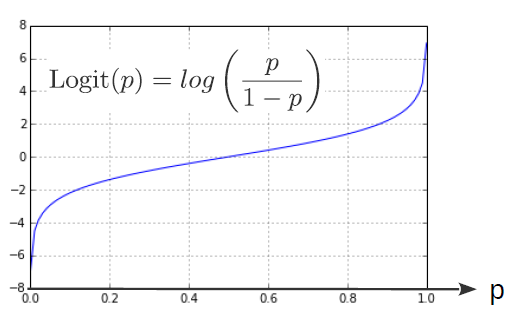
\includegraphics[width=70mm]{graphe1.png}
\end{minipage}
\hfill
\begin{minipage}[b!]{0.4\textwidth}
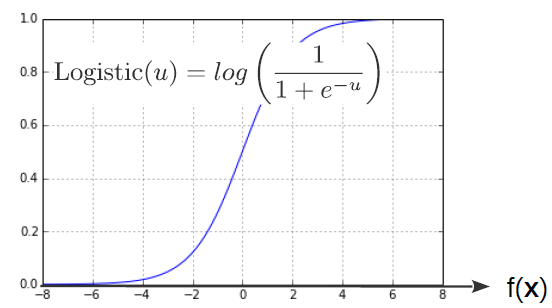
\includegraphics[width=70mm]{graphe2.png}
\end{minipage}
\end{figure}
\begin{center}
\(\log \dfrac{P(y=1|\xx)}{1 - P(y=1|\xx)} = \beta^T\xx + \beta_0\) with \(\beta = (\beta_0, ..., \beta_p)\)\\
\end{center}

\paragraph{Maximum likelihood estimation of logistic regression coefficients}

As usual, let's compute the log likelihood for this logistic regression, knowing our data \(\dd = {\{\xx^i,\textit{y}^i\}}_{\textit{i}=1,..,\textit{n}}\)  :\\
\\
\[\mathcal{L}(\beta|\dd) = \displaystyle\sum_{i=1}^{n} log P(y^i|\xx^i) + Cte = \displaystyle\sum_{i=1}^{n} (y^i \log g^i + (1-y^i) \log(1-g^i))\]
\begin{center}
with \(g = P(y=1|\xx) = \frac{1}{1+e^{-\beta^T\xx}}\) 
\end{center}
We find the maximum of the log-likelihood by calculating its gradient \(\nabla_{\beta}\mathcal{L}\): 

\[\nabla_{\beta}g^i = \xx^i g^i (1-g^i)\]

\[\nabla_{\beta}\mathcal{L} = \displaystyle\sum_{i=1}^{n} (y^i-g^i)\xx^i\]\\
\\
And solving for zero in the gradient formula :

\[\displaystyle\sum_{i=1}^{n} \left( y^i - \frac{1}{1 + e^{-\beta^T\xx^i}} \right) = 0\]\\
\\
However, this expression cannot be solved analytically. \\ Since $\mathcal{L}$ is concave, hence there is no local minima, we can use the gradient ascent method.
\\
\paragraph{Gradient ascent method} For a function J concave in $\beta$ :

\begin{itemize}
\item Update rule : \(\beta^{(t+1)} \leftarrow \beta^{(t)} + \eta \nabla_\beta J(\beta^{(t)})\)
\item Iterate until change is inferior to a chosen margin $\epsilon$
\item $\eta$ is the learning rate
\end{itemize}

\begin{center}
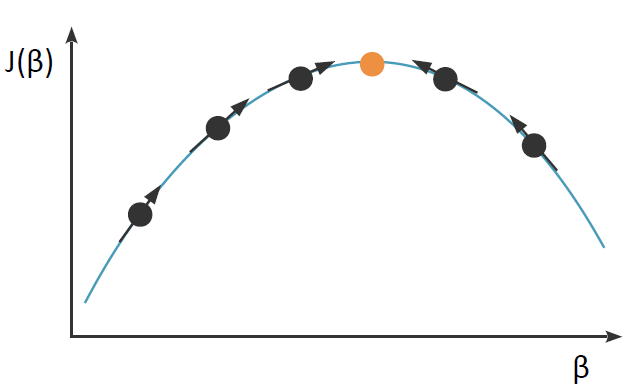
\includegraphics[width=100mm]{gradient.png}
\end{center}
Other methods remain possible such as the Newton method, conjugate gradient ascent or IRLS.


\section{Summary}

The main points to keep in mind from this lesson are the following : 
\begin{itemize}
\item MAP estimate : \(\hat{\theta}_{\mbox{MAP}}=\arg\underset{\theta}\max \  p(\theta|\mathcal{X})\)
\item MLE : \(\hat{\theta}_{\mbox{MLE}}=\arg\underset{\theta}\max \  p(\mathcal{X}|\theta)\)
\item Bayes estimate : \(\hat{\theta}_{\mbox{Bayes}}=\mathbb{E}[\theta|\mathcal{X}]=\int{\!\theta p(\theta|\mathcal{X})d\theta}\)
\item Assuming a Gaussian error, maximizing the likelihood (MLE) is equivalent to minimizing the RSS (residual sum of squares). 
\item Linear regression MLE : \(\hat{\beta} = (\textbf{\textit{X}}^T\textbf{\textit{X}})^{-1} \textbf{\textit{X}}^T y\) 
\item Logistic regression : to solve with gradient ascent. 
 \end{itemize}
\end{document}
